%! TeX root = master.tex
% !TEX program = lualatex

\lecture{6}{2026-10-15}{Applied cryptography continued}{}

\section{Recap and the two remaining problems}

\paragraph{What we have so far.} Last lecture solved \textbf{confidentiality}: Alice and Bob exchange $C = E_K(M)$ and Eve, who does not know $K$, cannot recover $M$. The whole security relies on the assumption that \textbf{Eve cannot access the secret key} (she cannot ``see inside the boxes'' doing encryption and decryption).
\begin{itemize}
    \item \textbf{Symmetric encryption} (OTP, stream ciphers): encryption and decryption use the \textbf{same pre-shared key} $K$.
    \item \textbf{Diffie--Hellman}: public parameters $p, g$; Alice sends $A = g^a \bmod p$, Bob sends $B = g^b \bmod p$; both compute $K = A^b = B^a = g^{ab} \bmod p$. Eve sees $A$ and $B$ but cannot recover $a$ or $b$ (\textbf{discrete logarithm problem}).
\end{itemize}

\paragraph{What is still missing.} This lecture solves two problems:
\begin{enumerate}
    \item \textbf{Problem I: Authenticity.} DH solves key distribution but creates the \textbf{identity verification problem}: how do Alice and Bob know they are talking to the right person, and not to Eve sitting in the middle (MITM)?
    \item \textbf{Problem II: Integrity.} Encryption alone does not prevent Eve from \textbf{modifying} the message (recall the bit-flipping attack on the OTP). How do we guarantee that if Bob sends ``Banana'', Alice receives ``Banana'' and not ``Apple''?
\end{enumerate}
Each problem is solved both in the \textbf{asymmetric} (public-key) setting and in the \textbf{symmetric} setting.

\section{Problem I: Authenticity (asymmetric cryptography)}

\subsection{Public-key cryptography}

\begin{definition}[Key pair]
In \textbf{asymmetric} (public-key) cryptography, every user owns \textbf{two keys}:
\begin{itemize}
    \item a \textbf{secret key} $SK$ (also called private key), that the user keeps to himself;
    \item a \textbf{public key} $PK$, that does \textbf{not} need to be secret and can be published.
\end{itemize}
Example in the DH setting (omitting the $\bmod p$): Alice has $SK_A = a$ and $PK_A = A = g^a$; Bob has $SK_B = b$ and $PK_B = B = g^b$.
\end{definition}

\begin{definition}[Public Key Infrastructure (PKI)]
The public keys are uploaded to \textbf{public servers} (repositories) that form the backbone of the \textbf{Public Key Infrastructure}. Anyone who wants to communicate with Alice fetches $PK_A$ from the PKI.
\end{definition}

\begin{center}
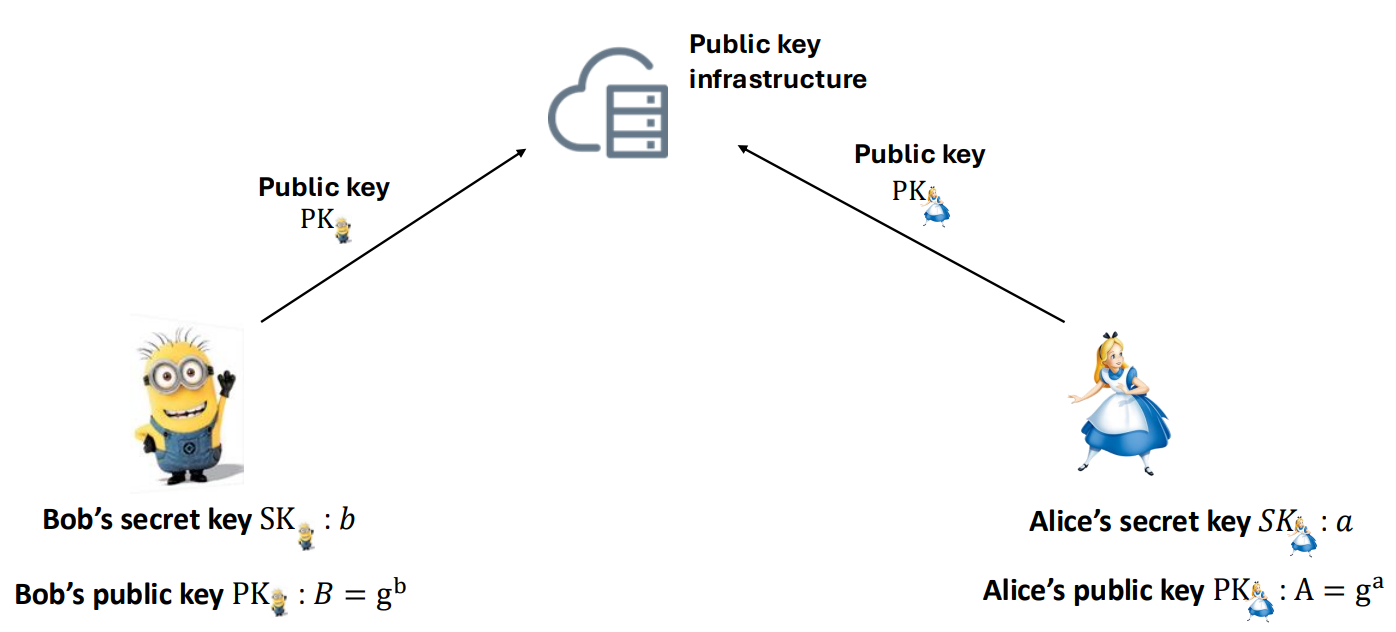
\includegraphics[width=0.9\linewidth]{images/img_20261101_124848.png}
\end{center}

\begin{remark}
The PKI must itself guarantee that ``$PK_A$ really belongs to Alice'': this is the role of the \textbf{Certificate Authorities} (CAs) mentioned last lecture. If Eve could substitute her own public key for Alice's in the repository, we would be back to a MITM. Integrity of the public keys bootstraps everything else.
\end{remark}

\subsection{Confidentiality: public-key encryption and decryption}

When Bob wants to write to Alice:
\begin{enumerate}
    \item Bob finds \textbf{Alice's public key} $PK_A$ in the repository;
    \item he encrypts the message with it: $C = E_{PK_A}(M)$;
    \item he sends the ciphertext $C$ to Alice;
    \item only Alice, with her \textbf{secret key}, can decrypt: $D_{SK_A}(C) = M$.
\end{enumerate}

\[
\boxed{C = E_{PK}(M), \qquad D_{SK}(C) = M}
\]
\begin{itemize}
    \item Decrypting with the \textbf{public} key returns garbage: $D_{PK}(C) \neq M$. This is what provides \textbf{confidentiality}: anyone can encrypt for Alice, but only Alice can decrypt.
    \item \textbf{Example} of standardised public-key encryption: \textbf{RSA-OAEP}.
    \item \textbf{Do not design your own}: always use standardised schemes for these boxes.
\end{itemize}

\begin{remark}[Classic exam trap]
One \textbf{never} decrypts a public-key ciphertext with the public key. In the Midterm 2024, answers claiming that $\mathrm{Enc}(PK_{\text{server}}, m)$ could be read by anyone ``because the server's public key is public'' got zero: encrypting under $PK$ is something anyone can do, decrypting requires $SK$.
\end{remark}

\subsection{Authenticity: digital signatures}

We follow the \textbf{same schema} to solve the identity verification problem, but with the roles of the keys swapped: the \textbf{secret} key is used to \emph{produce}, the \textbf{public} key to \emph{check}.

\begin{definition}[Digital signature scheme]
\begin{itemize}
    \item \textbf{Signing}: Bob uses his \textbf{secret signing key} $SK$ to compute a signature on the message:
    \[
    S = \mathrm{Sign}_{SK}(M).
    \]
    He sends $(M, S)$ to Alice.
    \item \textbf{Verification}: Alice fetches Bob's \textbf{public verification key} $PK$ from the PKI and runs
    \[
    V_{PK}(M, S) \in \{\text{yes}, \text{no}\}.
    \]
    \item \textbf{Correctness}: $V_{PK}\big(M, \mathrm{Sign}_{SK}(M)\big) = \text{yes}$ for every message $M$.
\end{itemize}
\end{definition}

\begin{definition}[Unforgeability: the security requirement]
It must be \textbf{impossible to forge a signature} $S$ on a message $M$ that verifies under $PK$ \textbf{without knowing the corresponding $SK$} (even after having seen signatures on many other messages).
\end{definition}

Under this property, a digital signature lets Alice know that she is talking to Bob: \textbf{only Bob, who knows $SK$, could have created the signature}. Example of standardised signature scheme: \textbf{NIST DSA}. Again: \textbf{do not design your own}.

\begin{remark}[Encryption vs.\ signature: which key does what]
\begin{center}
\begin{tabular}{@{}lll@{}}
\toprule
 & \textbf{Uses public key $PK$} & \textbf{Uses secret key $SK$} \\
\midrule
Encryption (confidentiality) & Encrypt (anyone, \emph{to} the owner) & Decrypt (only the owner) \\
Signature (authenticity) & Verify (anyone) & Sign (only the owner) \\
\bottomrule
\end{tabular}
\end{center}
The operation that must be \emph{restricted} is always the one done with the secret key.
\end{remark}

\subsection{The cost problem: sign the hash}

The convenience of not having to pre-share a key comes at a cost: asymmetric primitives are \textbf{computationally costly} compared with most symmetric algorithms of equivalent security, both for encryption and signing. Signing (and verifying) a long message directly would take far too long to be practical.

\textbf{Solution}: sign a short, fixed-size \textbf{digest} of the message, obtained with a \textbf{cryptographic hash function}.

\section{Hash functions}

\subsection{Definition}

\begin{definition}[Cryptographic hash function]
A cryptographic hash function $h(\cdot)$ is an \textbf{unkeyed} cryptographic primitive that takes as input a message $M$ of \textbf{any length} and outputs a \textbf{short, fixed-length} string of bits $H = h(M)$.
\begin{itemize}
    \item \textbf{Deterministic}: the same input always gives the same output.
    \item \textbf{Efficient}: designed to be fast to compute.
    \item \textbf{Unkeyed}: there is no secret involved; \emph{anyone} can compute $h(M)$ from $M$.
\end{itemize}
\end{definition}

\begin{remark}
Because $h$ is unkeyed and deterministic, a hash \textbf{alone} never provides integrity against an active adversary on the channel: if Eve replaces $M$ by $M'$, she can also replace $h(M)$ by $h(M')$. A hash protects integrity only when the hash value itself comes through a trusted channel (official website, inside a signature, \dots). Likewise, a hash is \textbf{not encryption}: if the input is guessable, anyone can recompute it.
\end{remark}

\subsection{The three security properties}

\begin{definition}[Pre-image resistance (one-wayness)]
Given a hash value $H = h(M)$, it is \textbf{difficult to find any} message $M'$ such that $h(M') = H$. In other words, hash functions are \textbf{not invertible}.
\end{definition}

\begin{definition}[Second pre-image resistance]
Given a message $M$ (and hence $h(M)$), it is \textbf{difficult to find another} message $M' \neq M$ such that $h(M') = h(M)$.
\end{definition}

\begin{definition}[Collision resistance]
It is \textbf{difficult to find any} pair of messages $M \neq M'$ such that $h(M) = h(M')$. Here the adversary chooses \emph{both} messages freely.
\end{definition}

\paragraph{Who chooses what?} The difference between the three properties is \textbf{what the adversary is given} and \textbf{what she is free to choose}:
\begin{center}
\begin{tabular}{@{}llll@{}}
\toprule
\textbf{Property} & \textbf{Adversary is given} & \textbf{Adversary must find} & \textbf{Free choice} \\
\midrule
Pre-image & a hash $H$ (arbitrary) & any $M'$ with $h(M') = H$ & $M'$ \\
Second pre-image & a message $M$ (arbitrary) & $M' \neq M$ with $h(M') = h(M)$ & $M'$ \\
Collision & nothing & $M \neq M'$ with $h(M) = h(M')$ & $M$ \emph{and} $M'$ \\
\bottomrule
\end{tabular}
\end{center}

\begin{remark}[Exam pitfalls on definitions (Midterm 2024 MRE)]
\begin{itemize}
    \item \textbf{Second pre-image is not ``given $h(M)$''.} In second pre-image resistance, the adversary is given the \textbf{input} $M$. If she only has $h(M)$ and finds an $M'$ with the same hash, that is a break of \textbf{(first) pre-image} resistance: breaking pre-image does not require finding the \emph{original} $M$, \textbf{any} input mapping to $H$ suffices.
    \item \textbf{Collisions always exist.} The input space is infinite (or at least much larger than the output space $\{0,1\}^n$), so by the \textbf{pigeonhole principle} collisions necessarily exist (e.g.\ a map from $2^{1024}$ values to $2^{512}$ values always has two inputs with the same output). The properties only state that collisions are \textbf{computationally hard to find}, never that they do not exist.
    \item \textbf{Second pre-image resistance is not ``to avoid collisions''.} It does not imply the absence of collisions, only that it is hard to find one \emph{for a given} $M$. And whether collisions matter depends on the threat model.
\end{itemize}
\end{remark}

\subsection{Standard hash functions}

As with any other primitive, designing good hash functions is hard: \textbf{do not design your own}, use standardised ones.
\begin{center}
\begin{tabular}{@{}lll@{}}
\toprule
\textbf{Function} & \textbf{Output size} & \textbf{Status} \\
\midrule
MD5 (1991) & 128 bits & \textbf{insecure} \\
SHA-0, SHA-1 & 160 bits & \textbf{insecure} \\
SHA-2 (SHA-224/256/384/512) & 224--512 bits & OK, but slow \\
SHA-3 (224/256/384/512) & 224--512 bits & OK (recommended) \\
\bottomrule
\end{tabular}
\end{center}

\subsection{Uses of hash functions}

Hash functions support \textbf{digital signatures}, are used to build \textbf{HMAC}, and serve for \textbf{password storage}, \textbf{file integrity} (checksums), \textbf{secure commitments}, \textbf{secure logging}, \textbf{blockchains}, \dots

\paragraph{Which property does an application need?} Always reason from the \textbf{threat model}: what is the adversary given, and what does she want to achieve?

\section{Digital signatures on hashes}

\subsection{The protocol}

To sign a message efficiently, \textbf{Bob}:
\begin{enumerate}
    \item hashes the message: $H = h(M)$;
    \item signs the hash: $S = \mathrm{Sign}_{SK}(H)$;
    \item sends to Alice the message \textbf{and} the signature on its hash: $(M, S)$.
\end{enumerate}
To verify the integrity and provenance of the message, \textbf{Alice}:
\begin{enumerate}
    \item recomputes $H = h(M)$ from the received message (since hashing is deterministic, she obtains the same $H$ as Bob);
    \item checks that the signature is valid on that hash: $V_{PK}(H, S) = \text{yes}$.
\end{enumerate}

\begin{center}
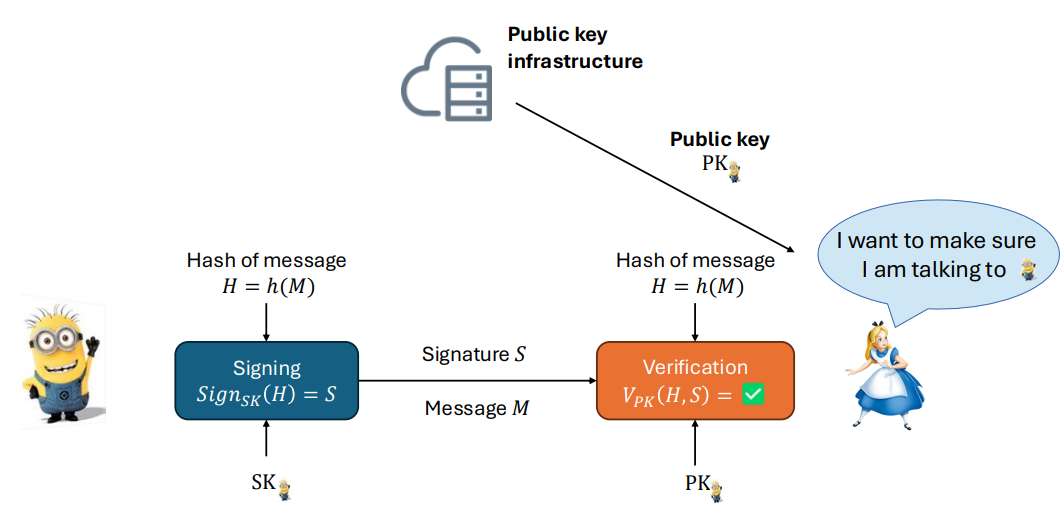
\includegraphics[width=0.8\linewidth]{images/img_20261101_133408.png}
\end{center}

\subsection{Which hash properties are needed?}

For signing $h(M)$ to be equivalent to signing $M$:
\begin{itemize}
    \item \textbf{Pre-image resistance: not needed}, because the message $M$ is sent \textbf{in the clear} anyway. There is nothing to hide in $h(M)$.
    \item \textbf{Second pre-image resistance: needed.} Given a signature on $h(M)$, an adversary must not be able to find another message $M' \neq M$ with $h(M') = h(M)$: otherwise the signature on $M$ would also be a valid signature on $M'$, and she could swap the message (forgery).
    \item \textbf{Collision resistance: needed.} Nobody (including the signer) must be able to produce two messages $M \neq M'$ with the same hash. Otherwise someone could have Bob sign the harmless $M$ and then claim that he signed $M'$ (or Bob could sign $M$ and later claim he signed $M'$).
\end{itemize}

\subsection{All together: confidentiality and authenticity in the asymmetric setting}

\begin{definition}[Asymmetric confidentiality + authenticity]
Users have \textbf{two key pairs}: one for encryption and one for signatures.
\begin{itemize}
    \item Encryption pair: public encryption key $PK^{\mathrm{enc}}$, secret decryption key $SK^{\mathrm{enc}}$;
    \item Signature pair: public verification key $PK^{\mathrm{sig}}$, secret signing key $SK^{\mathrm{sig}}$.
\end{itemize}
Bob sends to Alice:
\[
\boxed{E_{PK_A^{\mathrm{enc}}}(M), \quad \mathrm{Sign}_{SK_B^{\mathrm{sig}}}\big(h(M)\big)}
\]
\begin{itemize}
    \item \textbf{Confidentiality}: $D_{SK_A^{\mathrm{enc}}}(C) = M$ with $C = E_{PK_A^{\mathrm{enc}}}(M)$; only Alice can read.
    \item \textbf{Authentication}: $V_{PK_B^{\mathrm{sig}}}(h(M), S) = \text{yes}$ with $S = \mathrm{Sign}_{SK_B^{\mathrm{sig}}}(h(M))$; only Bob could have produced $S$.
\end{itemize}
Note that encryption uses the \textbf{receiver's} key and signing uses the \textbf{sender's} key.
\end{definition}

\begin{remark}
Here the message is encrypted, so the signature on $h(M)$ is sent next to a ciphertext. If $M$ is \textbf{guessable} (low entropy), an eavesdropper can hash every candidate and compare: $h(M)$ (and anything deterministic computed on the plaintext) can \textbf{leak the plaintext}. Keep this in mind for the composition analysis below and for the sensor exercise.
\end{remark}

\section{Problem II: Integrity}

\begin{definition}[Integrity]
\textbf{Integrity}: information \textbf{cannot be modified by unauthorized parties}. A cryptographic mechanism providing integrity must prevent Eve, sitting in the middle, from tampering with the ciphertext so that Alice decrypts ``Apple'' when Bob sent ``Banana'' \textbf{without this being detected}.
\end{definition}

\begin{center}
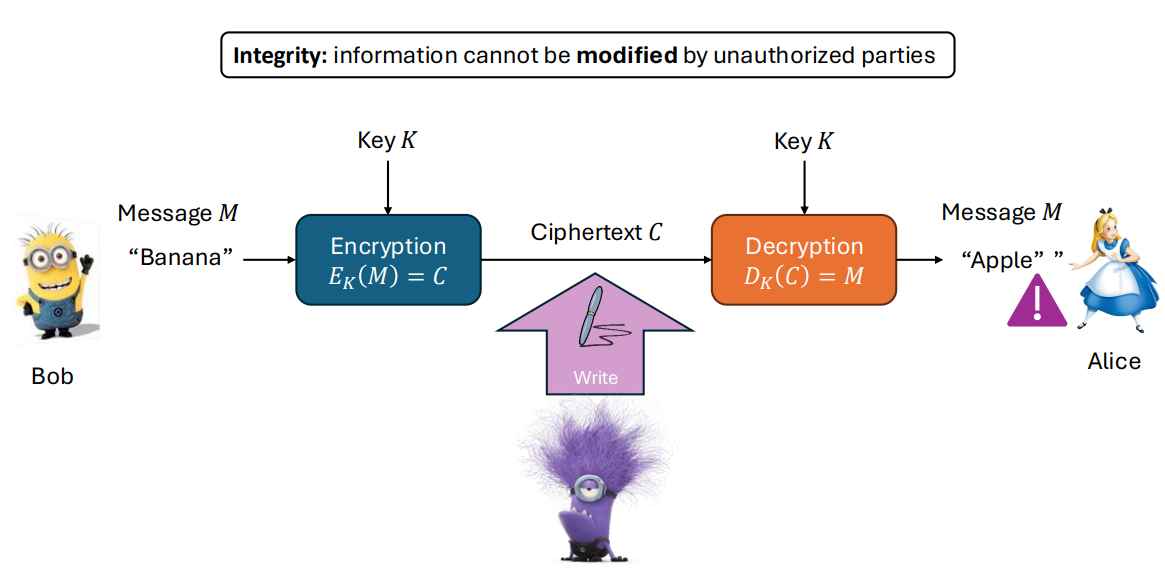
\includegraphics[width=0.9\linewidth]{images/img_20261101_135320.png}
\end{center}

\begin{remark}
Cryptography cannot \emph{prevent} Eve from changing bits on the wire; it can only make every modification \textbf{detectable}, so that the receiver rejects the message.
\end{remark}

\subsection{Integrity in the asymmetric setting: digital signatures}

We already have a solution: \textbf{digital signatures}. Since no party other than the sender can create a valid signature, signatures provide three properties:
\begin{itemize}
    \item \textbf{Sender authenticity}: no adversary can produce a valid signature under the sender's public key, so no adversary can impersonate the sender.
    \item \textbf{Message integrity}: an adversary cannot modify $M$ without being detected: if she modifies the message, the signature is no longer valid ($S$ only verifies if $M$ has not been modified).
    \item \textbf{Non-repudiation}: if a message has a valid signature, the sender \textbf{cannot claim that he did not sign it}, because no one else could have produced it. Anybody (including a \textbf{third party}, e.g.\ a judge) can verify this with the public key.
\end{itemize}

The rest of the lecture answers: \textbf{how do we provide integrity for symmetric exchanges} (pre-shared secret key)? The building block is the \textbf{block cipher}.

\section{Block ciphers and modes of operation}

\subsection{Block ciphers}

\begin{definition}[Block cipher]
A block cipher is a symmetric primitive that works on \textbf{small blocks} of fixed size (typically \textbf{128 or 256 bits}).
\begin{itemize}
    \item \textbf{Encryption} $E_K(M_i) = C_i$ takes the key and a message block, and outputs a ciphertext block of the \textbf{same size} as the input. The output \textbf{looks random}: it looks independent from the input.
    \item \textbf{Decryption} $D_K(C_i) = M_i$ is a (generally) \textbf{different} algorithm that, given the ciphertext block and the key, returns the plaintext block.
\end{itemize}
Example: \textbf{AES} (128-bit blocks; 128/192/256-bit keys).
\end{definition}

\paragraph{Problem.} Messages are longer than a block! We need to iterate the block cipher over the blocks $M = M_1 M_2 \dots M_n$. The way blocks are chained together is called a \textbf{mode of operation}.

\begin{remark}
In the lecture, all message blocks $M_i$ are assumed to have the size of one block (the last block is padded if needed).
\end{remark}

\subsection{Mode 1: Electronic Code Book (ECB)}

\begin{definition}[ECB]
The straightforward scheme: \textbf{encrypt and decrypt each block independently}.
\[
\boxed{C_i = E_K(M_i), \qquad M_i = D_K(C_i)}
\]
\end{definition}

\begin{center}
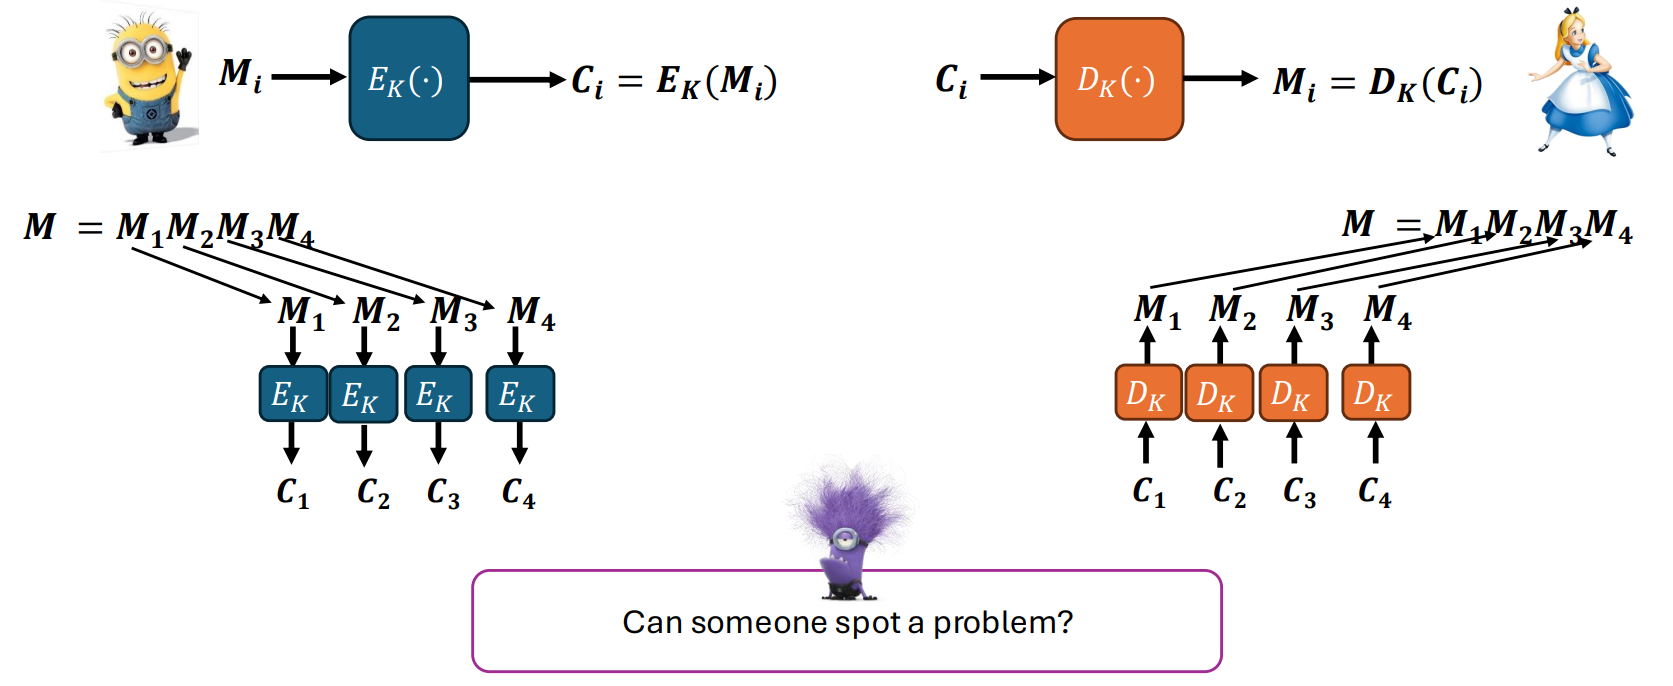
\includegraphics[width=0.8\linewidth]{images/img_20261101_153353.png}
\end{center}

\paragraph{The problem.} ECB is \textbf{deterministic per block}:
\[
\boxed{M_i = M_j \;\Longrightarrow\; C_i = C_j}
\]
If two blocks of the message are the same, they have the \textbf{same appearance} when encrypted. ECB therefore leaks the \textbf{structure} of the plaintext (which blocks repeat, and where): this is exactly the same flaw as the substitution cipher, at the level of blocks instead of letters. Encrypting the same message twice also gives the same ciphertext.

\begin{remark}
ECB also offers no integrity: Eve can \textbf{reorder, delete or duplicate} ciphertext blocks, and each one still decrypts to a valid plaintext block. Never use ECB for messages longer than one block.
\end{remark}

\subsection{Mode 2: Cipher Block Chaining (CBC)}

Idea: \textbf{add an IV and propagate information across blocks} to introduce randomness: each block's encryption depends on the previous ciphertext block.

\begin{definition}[CBC encryption]
\[
\boxed{C_0 = IV, \qquad C_i = E_K(M_i \oplus C_{i-1})}
\]
The ciphertext sent is $IV, C_1, C_2, \dots, C_n$.
\end{definition}

\begin{center}
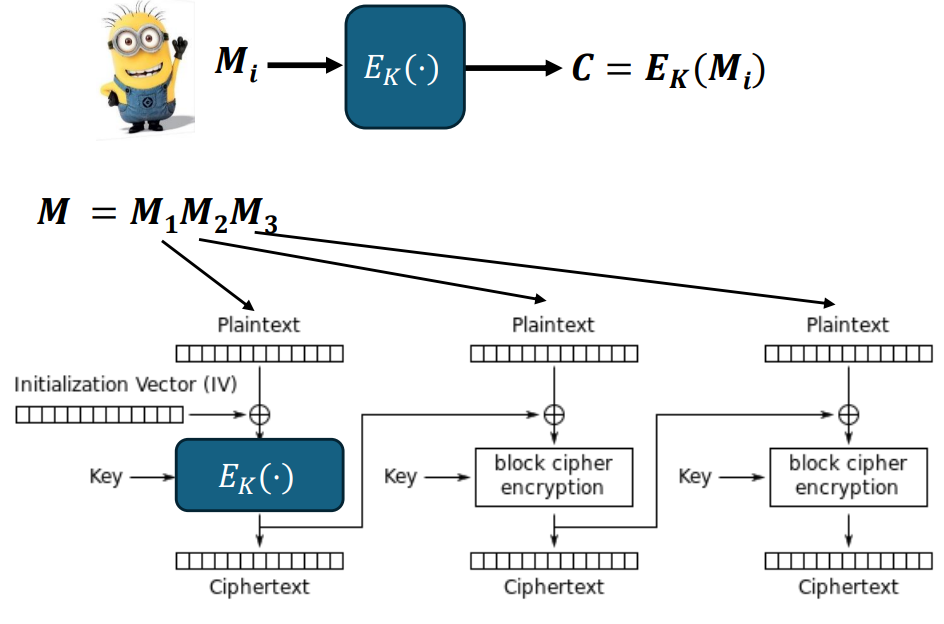
\includegraphics[width=0.6\linewidth]{images/img_20261101_153701.png}
\end{center}

\paragraph{Why it works.} By the properties of the block cipher, each ciphertext block looks random. Because the IV and/or the plaintext changes every time, this random value is different each time; XORing it with the next plaintext block before encryption acts like a \textbf{one-block one-time pad}. Equal plaintext blocks no longer give equal ciphertext blocks. But if one \textbf{reuses the IV} with the same key and the same plaintext, the same ciphertext is produced (and messages with a common prefix share the same first ciphertext blocks).

\begin{definition}[CBC decryption]
Inverse operation (note \emph{where} the XOR happens: \textbf{after} decryption):
\[
\boxed{C_0 = IV, \qquad M_i = D_K(C_i) \oplus C_{i-1}}
\]
\end{definition}

\begin{center}
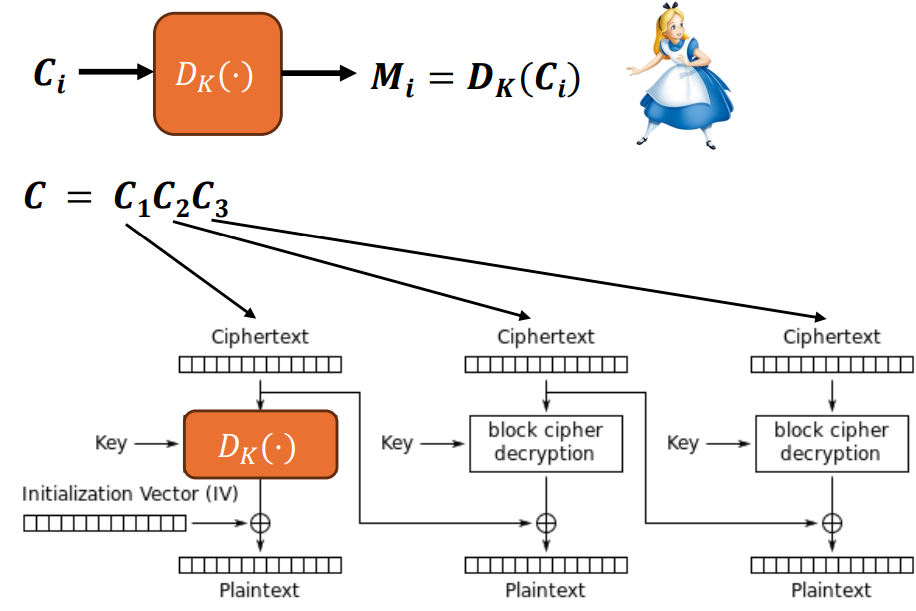
\includegraphics[width=0.6\linewidth]{images/img_20261101_153826.png}
\end{center}

\paragraph{Q1: what if the IV is incorrect? Is the full decryption wrong?} \textbf{No, only the first block is corrupted}: $M_1 = D_K(C_1) \oplus IV$ uses the IV, but every other block $M_i = D_K(C_i) \oplus C_{i-1}$ only depends on the \textbf{ciphertext}.

\paragraph{Q2: can you decrypt a block alone? What do you need?} A block cannot be decrypted without the \textbf{previous ciphertext block}: one needs $C_{i-1}$ to XOR with the output of $D_K(C_i)$. With $C_i$ and $C_{i-1}$ (and $K$), block $i$ can be decrypted on its own; one does \emph{not} need the previous plaintexts.

\paragraph{Additional properties (useful for exercises).}
\begin{itemize}
    \item \textbf{Encryption is sequential} ($C_i$ needs $C_{i-1}$), but \textbf{decryption can be parallelised} (all $C_i$ are known).
    \item \textbf{Error propagation}: a corrupted ciphertext block $C_i$ garbles the whole $M_i$ and flips the corresponding bits of $M_{i+1}$ (because $C_i$ is XORed into $M_{i+1}$); blocks after $i+1$ are fine.
    \item The IV is sent in the clear; it should be \textbf{unique and unpredictable} for each message.
\end{itemize}

\subsection{Mode 3: Counter mode (CTR)}

Idea: \textbf{use an increasing nonce} to add randomness \textbf{without dependencies between blocks}.

\begin{definition}[Nonce]
A \textbf{nonce} is a ``\textbf{n}umber used only \textbf{once}'': it must be \textbf{new for every message} (under a given key).
\end{definition}

\begin{definition}[CTR encryption and decryption]
\[
\boxed{C_i = E_K(\mathrm{Nonce} + i) \oplus M_i, \qquad M_i = E_K(\mathrm{Nonce} + i) \oplus C_i}
\]
The block cipher encrypts the unique number $\mathrm{Nonce} + i$ (nonce and counter); the output is a random-looking \textbf{one-time pad} that is XORed with the plaintext. The counter keeps increasing, so that, if the nonce is new, the output of the block cipher is different for every block.
\end{definition}

\begin{center}
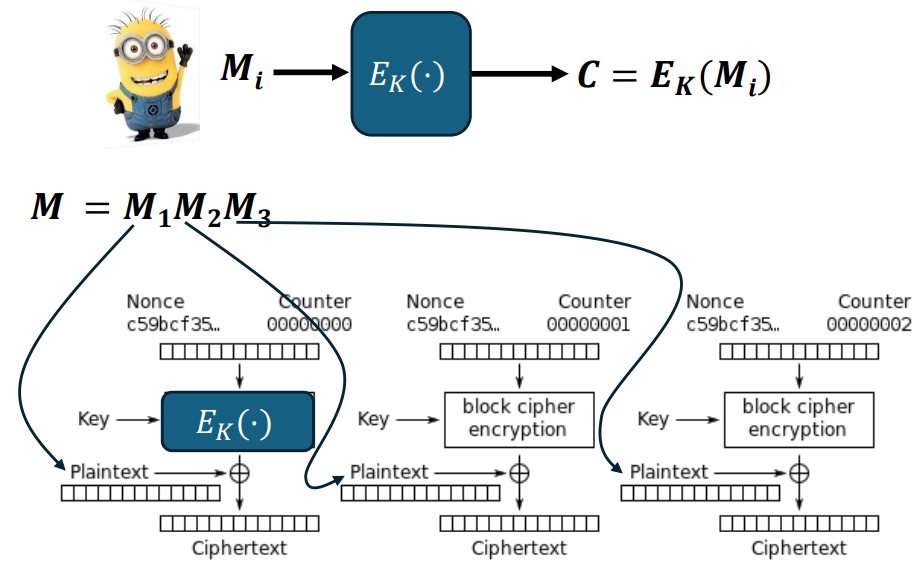
\includegraphics[width=0.6\linewidth]{images/img_20261101_154330.png}
\end{center}

\paragraph{Do we need a decryption algorithm?} \textbf{No.} CTR operates like a one-time pad (a \textbf{stream cipher} built from a block cipher: the keystream is $E_K(\mathrm{Nonce}+1), E_K(\mathrm{Nonce}+2), \dots$). To decrypt, one needs the same pseudo-random sequence, which is obtained with the same algorithm: \textbf{encryption} $E_K$. $D_K$ is never used.

\begin{center}
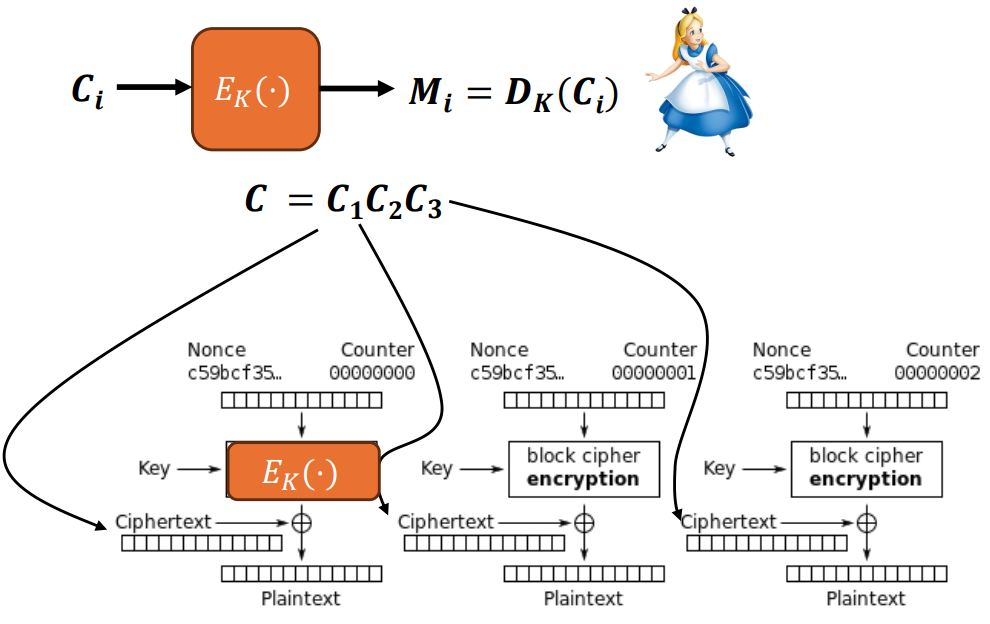
\includegraphics[width=0.6\linewidth]{images/img_20261101_154500.png}
\end{center}

\paragraph{Nonce reuse.} If the nonce is reused with the same key, the block cipher receives the same inputs and produces the same keystream: we are effectively \textbf{reusing a one-time pad}, and $C \oplus C' = M \oplus M'$ (see last lecture).

\paragraph{Additional properties.}
\begin{itemize}
    \item Blocks are independent: \textbf{parallel encryption and decryption}, and \textbf{random access} (decrypt block $i$ alone with only $C_i$, the nonce and $i$).
    \item \textbf{No error propagation}: a flipped bit in $C_i$ flips exactly the same bit in $M_i$.
    \item But, like any stream cipher, CTR is \textbf{malleable}: $C_i \oplus \Delta$ decrypts to $M_i \oplus \Delta$. CTR gives \textbf{no integrity} on its own.
    \item The nonce only needs to be unique, not secret or unpredictable (it is sent with the ciphertext).
\end{itemize}

\subsection{Block ciphers: strengths and weaknesses}

\begin{table}[h]
\centering
\begin{tabular}{@{}p{4.2cm}p{9.2cm}@{}}
\toprule
\multicolumn{2}{@{}l}{\textbf{Strengths}} \\
\midrule
High diffusion & Information from one plaintext symbol is diffused into several ciphertext symbols (chaining entangles blocks: every bit affects several blocks). \\
Immunity to tampering & Difficult to insert symbols without detection: a modification propagates, and the decryption no longer makes sense. \\
\midrule
\multicolumn{2}{@{}l}{\textbf{Weaknesses}} \\
\midrule
Slow & An entire block must be accumulated before encryption/decryption can begin (compared to stream ciphers, which work bit by bit). \\
Error propagation & In some modes (e.g.\ CBC, where encryption is chained), errors affect several bits/blocks. \\
\bottomrule
\end{tabular}
\caption{Block ciphers vs.\ stream ciphers. Note it is the exact mirror of the stream cipher table of last lecture. \emph{Individual modes may not fall in these categories} (e.g.\ CTR behaves like a stream cipher: low diffusion, no error propagation).}
\end{table}

\section{Message Authentication Codes (MAC)}

Back to the original problem: integrity for \textbf{symmetric} exchanges, where Alice and Bob share a secret key $K$.

\subsection{Definition}

\begin{definition}[Message Authentication Code]
A MAC takes two inputs:
\begin{itemize}
    \item a \textbf{fixed-size (short) secret key} $K$;
    \item the \textbf{message} $M$ whose integrity must be secured;
\end{itemize}
and outputs a \textbf{short} string $\mathrm{MAC}_K(M)$ (the \emph{tag}).

\textbf{Security property}: it is \textbf{hard to generate a pair} $\{M, \mathrm{MAC}_K(M)\}$ (for a new message $M$) \textbf{without knowing $K$}.
\end{definition}

\paragraph{Protocol.}
\begin{enumerate}
    \item Bob and Alice have a \textbf{pre-shared secret key} $K$.
    \item Bob computes $\mathrm{MAC}_K(M)$ and sends $\{M; \mathrm{MAC}_K(M)\}$.
    \item Alice recomputes $\mathrm{MAC}_K(M)$ on the received message with her copy of $K$ and \textbf{compares} it to the received tag. If they are equal, the message has not been tampered with; otherwise she rejects it.
\end{enumerate}

\paragraph{Two properties.}
\begin{enumerate}
    \item \textbf{$M$ cannot be tampered with} (integrity): a modified message would need a new valid tag, which Eve cannot compute without $K$.
    \item \textbf{The message comes from Bob/Alice} (authenticity): since only Alice and Bob know $K$, a message with a valid MAC could only have been written by one of them.
\end{enumerate}

\begin{remark}[MAC vs.\ hash]
A MAC is a \textbf{keyed} function, a hash is \textbf{unkeyed}. This is precisely why a MAC gives integrity over an insecure channel and a hash does not: Eve can recompute $h(M')$ for her modified message, but not $\mathrm{C}_K(M')$.
\end{remark}

\begin{remark}[Exam reminders on MACs]
\begin{itemize}
    \item \textbf{A MAC is a symmetric primitive.} When working with asymmetric keys, integrity is provided by \textbf{digital signatures}, never by a ``MAC with a public key'' (penalised in the Midterm 2024).
    \item The guarantee comes \textbf{from the secrecy of $K$}: always mention the key when justifying integrity.
    \item \textbf{Brute-forcing the MAC key is infeasible}: even if the message space is small and the MAC is deterministic, $K$ comes from a cryptographically large key space (by construction). Collecting many $(M, \mathrm{MAC}_K(M))$ pairs does not help recover $K$.
    \item A MAC is \textbf{deterministic} (same $K$, same $M$ $\Rightarrow$ same tag) and is \textbf{not designed for confidentiality}: the tag may leak information on $M$ (at least equality of messages).
\end{itemize}
\end{remark}

\subsection{MACs do not provide non-repudiation}

MACs give \textbf{mutual authentication}, but \textbf{no sender authenticity towards a third party}.

\begin{example}[Repudiation]
Bob sends Alice $\{M = \text{``I don't like Charlie''};\ \mathrm{MAC}_K(M)\}$ and Charlie (a third party) sees it. Alice and Bob know they are talking to each other: only a party knowing $K$ could produce a valid pair. But \textbf{both} of them know $K$, so both could have produced it:
\begin{itemize}
    \item Bob: ``I never wrote that message. It was Alice.''
    \item Alice: ``I never wrote that message. It was Bob.''
\end{itemize}
Charlie cannot decide: the message can be \textbf{repudiated}. Moreover, Charlie cannot even verify the MAC without $K$.
\end{example}

\begin{center}
\begin{tabular}{@{}lcc@{}}
\toprule
 & \textbf{MAC} (symmetric) & \textbf{Digital signature} (asymmetric) \\
\midrule
Key(s) & one shared secret $K$ & $SK$ to sign, $PK$ to verify \\
Integrity & yes & yes \\
Authenticity (to the other party) & yes & yes \\
Verifiable by a third party & no (needs $K$) & yes (with $PK$) \\
Non-repudiation & \textbf{no} & \textbf{yes} \\
Speed & fast & slow \\
\bottomrule
\end{tabular}
\end{center}

\subsection{Example MAC: CBC-MAC}

A block cipher can be turned into a MAC by running \textbf{CBC with a fixed IV} and keeping only the last block.

\begin{definition}[CBC-MAC]
\[
\boxed{C_0 = 0 \ \text{(any fixed IV)}, \qquad C_i = E_K(M_i \oplus C_{i-1}), \qquad \mathrm{MAC}_K(M_1 \dots M_n) = C_n}
\]
The last block can only have been reached for this message and this key, and it reveals nothing about the message (it looks random, as it is the output of a block cipher).
\end{definition}

\section{Authenticated encryption: confidentiality and integrity together}

How do we combine a symmetric encryption scheme ($\mathrm{Enc}$) and a MAC to obtain \textbf{both} confidentiality and integrity? There are three generic compositions (Bellare \& Namprempre, 2000).

\subsection{Encrypt-and-MAC}

\begin{center}
  
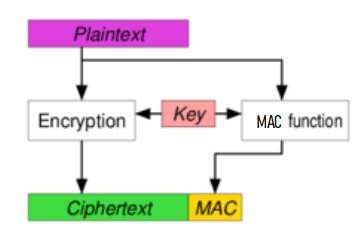
\includegraphics[width=0.3\linewidth]{images/img_20261101_160213.png}
\end{center}

\[
\mathrm{Enc}_{K_1}(M), \ \mathrm{MAC}_{K_2}(M)
\]
The MAC is computed on the \textbf{plaintext} and sent in the clear next to the ciphertext.
\begin{itemize}
    \item[$-$] \textbf{No integrity on the ciphertext}: the ciphertext can be attacked (the MAC does not protect it); one \textbf{needs to decrypt} (expensive) to know whether the message is valid.
    \item[$+$] Integrity of the \textbf{plaintext} can be verified.
    \item[$-$] \textbf{May reveal information about the plaintext}: the MAC is deterministic (recall the fixed IV of CBC-MAC) and visible, so if the same message is sent twice, the MAC is the same for both. (Can be mitigated by including a counter in the MAC input.)
\end{itemize}

\subsection{MAC-then-Encrypt}
\begin{center}
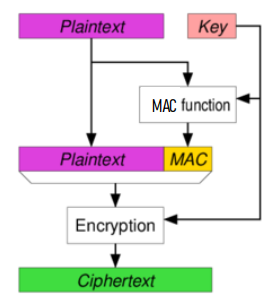
\includegraphics[width=0.3\linewidth]{images/img_20261101_160600.png}
\end{center}

\[
\mathrm{Enc}_{K_1}\big(M \,\|\, \mathrm{MAC}_{K_2}(M)\big)
\]
The MAC is computed on the plaintext, then the plaintext and its MAC are encrypted together.
\begin{itemize}
    \item[$-$] \textbf{Still no integrity of the ciphertext}: (in theory) it is possible to change the ciphertext and still have a valid MAC; one \textbf{needs to decrypt} to know whether the message is valid.
    \item[$+$] Integrity of the plaintext can be verified.
    \item[$+$] \textbf{No information on the plaintext} from the MAC, since the adversary does not see it (it is inside the encrypted blob).
\end{itemize}

\subsection{Encrypt-then-MAC}
\begin{center}  
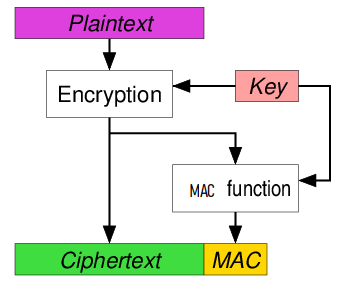
\includegraphics[width=0.3\linewidth]{images/img_20261101_160716.png}
\end{center}

\[
\boxed{C = \mathrm{Enc}_{K_1}(M), \quad \mathrm{MAC}_{K_2}(C)}
\]
The MAC is computed on the \textbf{ciphertext}.
\begin{itemize}
    \item[$+$] \textbf{Integrity of the ciphertext}: the receiver checks the MAC \textbf{before decrypting} and rejects anything modified. This ensures you \textbf{only read (decrypt) valid messages}; the cipher cannot be attacked (e.g.\ no bit flipping on CTR, no malleability).
    \item[$+$] Integrity of the plaintext can be verified (a valid ciphertext decrypts to the intended plaintext).
    \item[$+$] \textbf{No information on the plaintext}: the MAC is computed on the ciphertext, which already looks random.
\end{itemize}
\textbf{Encrypt-then-MAC is the recommended composition.}

\begin{table}[h]
\centering
\begin{tabular}{@{}lccc@{}}
\toprule
 & \textbf{Ciphertext integrity} & \textbf{Plaintext integrity} & \textbf{No leak via MAC} \\
\midrule
Encrypt-and-MAC & $\times$ & $\checkmark$ & $\times$ \\
MAC-then-Encrypt & $\times$ & $\checkmark$ & $\checkmark$ \\
Encrypt-then-MAC & $\checkmark$ & $\checkmark$ & $\checkmark$ \\
\bottomrule
\end{tabular}
\caption{Generic compositions of encryption and MAC.}
\end{table}

\begin{remark}[Use two different keys]
Use \textbf{independent keys} $K_1$ for encryption and $K_2$ for the MAC. Reusing the same key for two different primitives can create unexpected interactions between them (e.g.\ CBC encryption and CBC-MAC with the same key).
\end{remark}

\begin{example}[MCQ Midterm 2023: Roberta and Gustave]
Roberta and Gustave have securely pre-shared two symmetric keys $K_1, K_2$. Which option ensures \textbf{confidentiality and integrity}?
\begin{itemize}
    \item $\mathrm{Enc}(K_1, m), \mathrm{MAC}(K_1, m)$: same key for both, Encrypt-and-MAC: $\times$.
    \item $\mathrm{Enc}(K_1, m), \mathrm{MAC}(K_2, m)$: Encrypt-and-MAC, no ciphertext integrity, deterministic MAC leaks: $\times$.
    \item $\mathrm{MAC}(K_2, \mathrm{Enc}(K_1, m))$: only the tag is sent, Gustave cannot recover $m$ (a MAC is not invertible): $\times$.
    \item $\mathbf{Enc(K_1, m), MAC(K_2, Enc(K_1, m))}$: \textbf{Encrypt-then-MAC with two keys}: $\checkmark$.
\end{itemize}
\end{example}

\section{Conclusions: what we have learned about applied cryptography}
\begin{table}[h]
\centering
\begin{tabular}{@{}p{3.2cm}p{6.3cm}p{6.3cm}@{}}
\toprule
 & \textbf{Confidentiality} & \textbf{Integrity / Authentication} \\
\midrule
\raggedright \textbf{Symmetric} (shared $K$) & \raggedright Stream ciphers, block ciphers (+ modes of operation) & \raggedright Message Authentication Codes (MACs) \tabularnewline
\addlinespace
\raggedright \textbf{Asymmetric} ($PK$, $SK$) & \raggedright Public-key encryption ($E_{PK}$, $D_{SK}$) & \raggedright Digital signatures ($\mathrm{Sign}_{SK}$, $V_{PK}$) \tabularnewline
\bottomrule
\end{tabular}
\caption{The applied cryptography toolbox.}
\end{table}

\textbf{Hash functions}: three security properties (pre-image, second pre-image, collision resistance); they support digital signatures and many other functions.

